\chapter{\introduction}
\label{cha:Intro}

La inclusión del Smartphone se ha extendido hasta el punto de ser una herramienta indispensable en el día a día, tanto para comunicación \cite{Montag2015}, como para la búsqueda de información \cite{Wang2016}. El uso del Smartphone en estos aspectos está superando a los sistemas de cómputo tradicionales como el PC o los portátiles. El Smartphone dispone actualmente una capacidad de trabajo similar a los PC, con la ventaja de la movilidad que ofrece. En la actualidad, con un Smartphone se pueden realizar la mayoría de tareas cotidianas que un usuario puede requerir, como leer el correo electrónico, comunicarse con sus seres queridos, consultar información en la web o realizar compras online.

La característica principal del Smartphone es la movilidad que ofrece frente a los PC o portátiles tradicionales. A pesar de las ventajas que ofrece, el uso de dispositivos móviles, estos acarrean la inclusión de nuevos factores que pueden dificultar su usabilidad \cite{zhang2005challenges} como son:
\begin{itemize}
	\item \textbf{Contexto móvil}: el usuario puede cambiar su localización durante su uso. Asimismo, esto puede incluir interacción con su entorno, personas, objetos o el ambiente más próximo.
	\item \textbf{Conectividad}: la conectividad de los dispositivos móviles es lenta y poco fiable.
	\item \textbf{Tamaño de la pantalla}: la cantidad de información que se puede mostrar se reduce debido al tamaño de la pantalla que llega a un máximo de 7`` (los conocidos como phablets\footnote{Los phablet son dispositivos móviles denominados de esta manera por comprenderse en un tamaño mayor que los smartphones (hasta 5") y menor que los tablets (a partir de 7"): \url{https://en.wikipedia.org/wiki/Phablet}}).
	\item \textbf{Limitación de procesamiento}: los dispositivos móviles debido a su reducido tamaño disponen de menor capacidad de cómputo, lo que reduce el número de aplicaciones que son adecuadas para móviles.
	\item \textbf{Métodos de entrada de datos}: los dispositivos móviles ofrecen una peor usabilidad a la hora de introducir datos, el teclado táctil, los gestos y la voz son menos precisos y la inclusión de datos erróneos se incrementa \cite{Flood2011Tedious}. 
\end{itemize}

Debido a estas limitaciones, resulta complejo el uso de algunas aplicaciones en dispositivos móviles. Entre ellas destaca las hojas de cálculo, que son complejas debidas a las limitaciones de los Smartphone previamente descritas \cite{Flood2010}.

En la actualidad el uso de hojas de cálculo como Microsoft Excel o Google Spreadsheet es una de las herramientas más utilizadas en el manejo de información, en el ámbito empresarial, pero también a nivel personal. La potencia y versatilidad que ofrece es de sobra conocida, de ahí que exista gran cantidad de hojas de cálculo para el almacenamiento de datos. Actualmente cerca de 750 millones de usuarios utilizan Microsoft Excel para presentar y analizar datos \cite{Investitech2015}.

Un estudio reciente ha demostrado que el 79\% de los participantes (seleccionados a traves del European Spreadsheet Risk Interest Group\footnote{Sitio web de EuSpRiG: \url{http://www.cimaglobal.com/Thought-leadership/Newsletters/Insight-e-magazine/Insight-Archive/Are-you-managing-your-spreadsheet-risk/}} \footnote{¿Cuáles son los riesgos de las hojas de cálculo? \url{http://www.cimaglobal.com/Thought-leadership/Newsletters/Insight-e-magazine/Insight-Archive/Are-you-managing-your-spreadsheet-risk/}}) requieren de acceso a hojas de cálculo en una configuración móvil \cite{Flood2011SpreadsheetsMove}, especialmente en estos contextos de uso:
\begin{itemize}
	\item En el día a día o tareas cotidianas
	\item Demostración de datos a clientes
	\item Cuando reciben un correo electrónico con una hoja de cálculo (dado que es el medio de compartición favorito para las hojas de cálculo).
	\item A la hora de debatir cambios urgentes con compañeros de trabajo.
\end{itemize}

Tal y como se puede apreciar en este estudio, el uso de las hojas de cálculo en una configuración móvil es diferente a la que se presenta en el uso de los ordenadores tradicionales. El uso más habitual es el de consultar o modificar datos de hojas de cálculo ya existentes, es decir, que rara vez se diseñan hojas de cálculo nuevas, o se cambia gran cantidad de información de las mismas.

Una vez conocidos los usos más habituales de las hojas de cálculo en un entorno móvil y las limitaciones del Smartphone, \textbf{¿Cuáles son las razones por las que resulta complejo interactuar con ellas en un entorno móvil?}.

El limitado tamaño de la pantalla obliga al usuario a realizar muchas más interacciones cuando esta visualizando extensas hojas de cálculo. Esto provoca dos problemas \cite{Flood2011Tedious}:
\begin{itemize}
	\item \textbf{Usabilidad pobre o limitada}: En la Figura \ref{fig:MobileSheetScrolling} se presentan dos imágenes de una hoja de cálculo. Cada fila representa a un alumno y cada columna un parcial de una asignatura concreta. Como se puede observar, resulta tedioso obtener los exámenes de un alumno dado que hay que ir haciendo scrolling a lo largo de la hoja y rápidamente se pierde el foco de en qué fila está el dato asociado a ese alumno.
	\item \textbf{Sobrecarga cognitiva}: Los usuarios, debido a que solo pueden ver pequeñas porciones de la hoja de cálculo, tienen dificultades para conceptualizar la hoja de cálculo y como casa la porción que están visualizando en el conjunto global de la hoja.
\end{itemize}

\begin{figure}[htb]
	\centering
	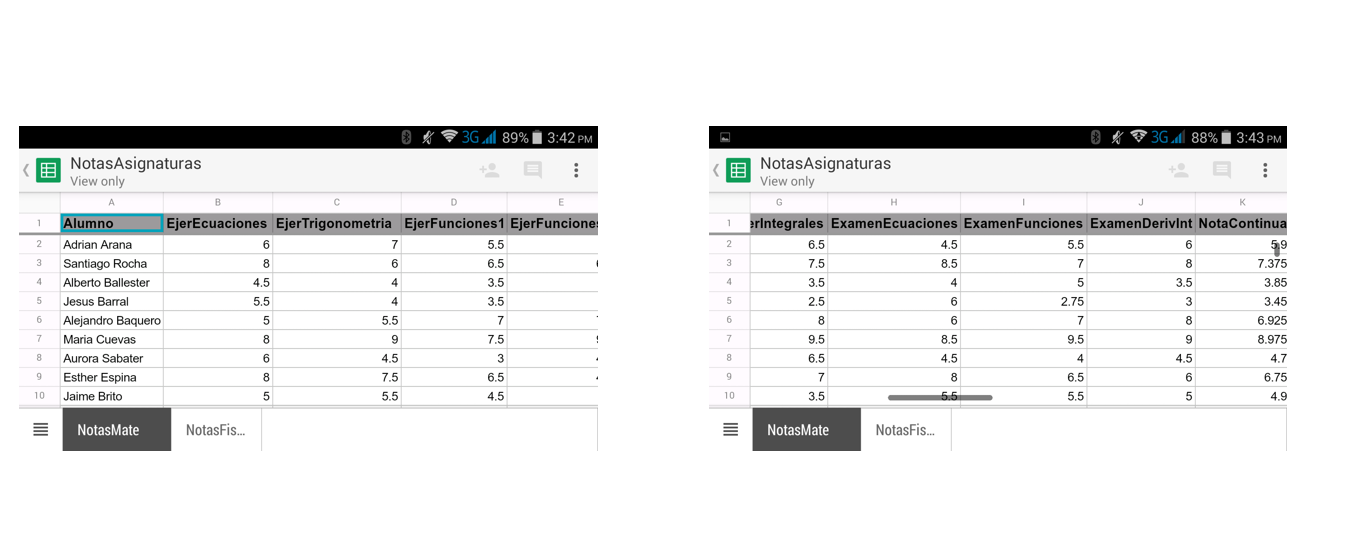
\includegraphics[width=0.8\textwidth]{./figs/MobileSheetScrolling.png}
	\caption{El problema de visualización de hojas de cálculo en dispositivos móviles debido al scrolling.}
	\label{fig:MobileSheetScrolling}
\end{figure}

La idea principal de este trabajo se apoya en dos premisas:
\begin{itemize}
	\item \textbf{Hay usuarios que trabajan con hojas de cálculo en entornos móviles}, especialmente para la consulta de los datos. La solución debe de ir enfocada a usuarios como son los comerciales, administrativos, analistas,... que son los que principalmente hacen uso de esta herramienta en entornos móviles.
	
	\item \textbf{El acceso con el dispositivo móvil a las hojas de cálculo es complejo} o farragoso con las aplicaciones actualmente existentes (como Microsoft Excel \footnote{Sitio web de las aplicaciones móviles de Microsoft Excel: \url{https://products.office.com/en/mobile/office}} o Google Sheets \footnote{Sitio web de descarga de Google SpreadSheets para Android e iOS: \url{https://www.google.com/mobile/drive/}}). Sin embargo, como se ha mencionado previamente, el uso de las aplicaciones de chat se han adaptado perfectamente al día a día de los usuarios y están muy extendidas dentro de los dispositivos móviles. Son utilizadas principalmente para hablar con seres queridos o compañeros de trabajo \cite{Montag2015}, aunque también está creciendo el uso para interactuar con Chatbots \footnote{Tendencia de interés respecto al término ``chatbot'' en Google Trends: \url{https://www.google.com/trends/explore?q=chatbot}}. Un Chatbot es un software capaz de resolver preguntas sobre un ámbito concreto realizadas en una interfaz textual. Se puede encontrar una introducción a los Chatbots en el Capítulo \ref{cha:IntroChatbot}.
\end{itemize}

Por lo tanto, la pregunta a la que se trata de dar respuesta en este trabajo es \textbf{¿Cómo se puede utilizar un Chatbot como interfaz para extraer la información que un usuario requiere?}. Para ello este documento presenta el trabajo bibliográfico y de investigación que se ha desarrollado entorno a la generación de Chatbots para autoconsumo utilizando hojas de cálculo. En este Capítulo \ref{cha:Intro} se ha presentado el contexto en el que se desarrolla el proyecto y el problema a resolver. En el Capítulo \ref{cha:IntroChatbot} se presenta una introducción a los Chatbots, que son la interfaz de consulta que se utilizará para acceder a las hojas de cálculo. En el Capítulo \ref{cha:AnalysisAndDesign} se analizarán los requisitos y las características que debe de tener el artefacto a implementar para resolver la problemática sobre la que se sostiene este trabajo. En el Capítulo \ref{cha:Implementation} se hace hincapié en la implementación y las tecnologías utilizadas para el desarrollo del software. En el Capítulo \ref{cha:CaseStudies} se presentan tres casos de estudio para evaluar la aplicabilidad de la solución adoptada. Finalmente en el Capítulo \ref{cha:Conclusions} se presenta el trabajo futuro que se va a realizar en el contexto de este trabajo y las conclusiones extraídas del mismo.